
\section{Auctions}
\label{w-auctions}

    Consider a case in which the option seller, only has one kind of asset and wants to sell options in different kind of assets (different kind of coins). He can do the change in two different manners: 1- make a chain of swaptions 2- put a ratio to handle currency fluctuations and at the time of exercising the option, put the ratio into an auction to convert it to needed currency (Bcoin).

    The second scenario seems rational if the option seller is a big deep market of cryptocurrencies and can afford to put principals more than the equivalent counter party's principal, but in another cryptocurrency.
    As an instance, imagine Bob is the option seller and all his asset is in Bcoins. Alice is the option buyer and her asset is in Acoins which she wants to swap with some Ccoins. Bob enters a swaption with Alice which exchanges Acoins with Bcoins. This is not what Alice really wanted (she needed Ccoins), so Bob should put more Bcoins in order to handle future changes in value of assets. At the time of exercising the option, Bob's money will be sent to a atomic swap with a very short duration and a secret that is owned by Bob. Because of the short locktimes, the premium needed in atomic swap is negligible. The counter party of the atomic swap also is Bob and he is given this short opportunity to change the Bcoins, with the amount of Ccoins Alice had requested. If Bob fails to provide Alice with needed Ccoins, Alice would swap Bcoins with her needed asset in other swaptions or atomic swaps. As Bcoins where over-collateralized, this would be easy for Alice to do so.
    



% This bond is not collateralized so there should be no margin in the borrower (Alice) side. 
% Additionally, Bob has the margin so he can not default after receiving premium, because Alice will take the margin.
% To convince Bob to reveal K1, Alice gives him the NOINPUT transaction which is locked with K1 and they both sign it. Just like swaptions, the Safe Box is signed by Alice and Bob and Carol, the next party that Alice is going to trade with using the bond. 
By using the above form, we can offer decentralized non-collateralized bond to parties that are in the same blockchain, because the anti-cheat transaction has inputs from both Alice's and Bob's sides. For overcoming this issue, before settling any bond contract Bob, which is considered to be an exchange or somebody who has reasonable amount of money in different chains, can deposit some money in every desired chain as a bond guarantee equal to the punishment amount. In this way, Bob can offer his customers a crosschain bond service which accepts his payback money in the other chain. This modification can be seen in Fig.\ref{fig:cross-chain-non-collat-bond}


\begin{figure}
    \centering
    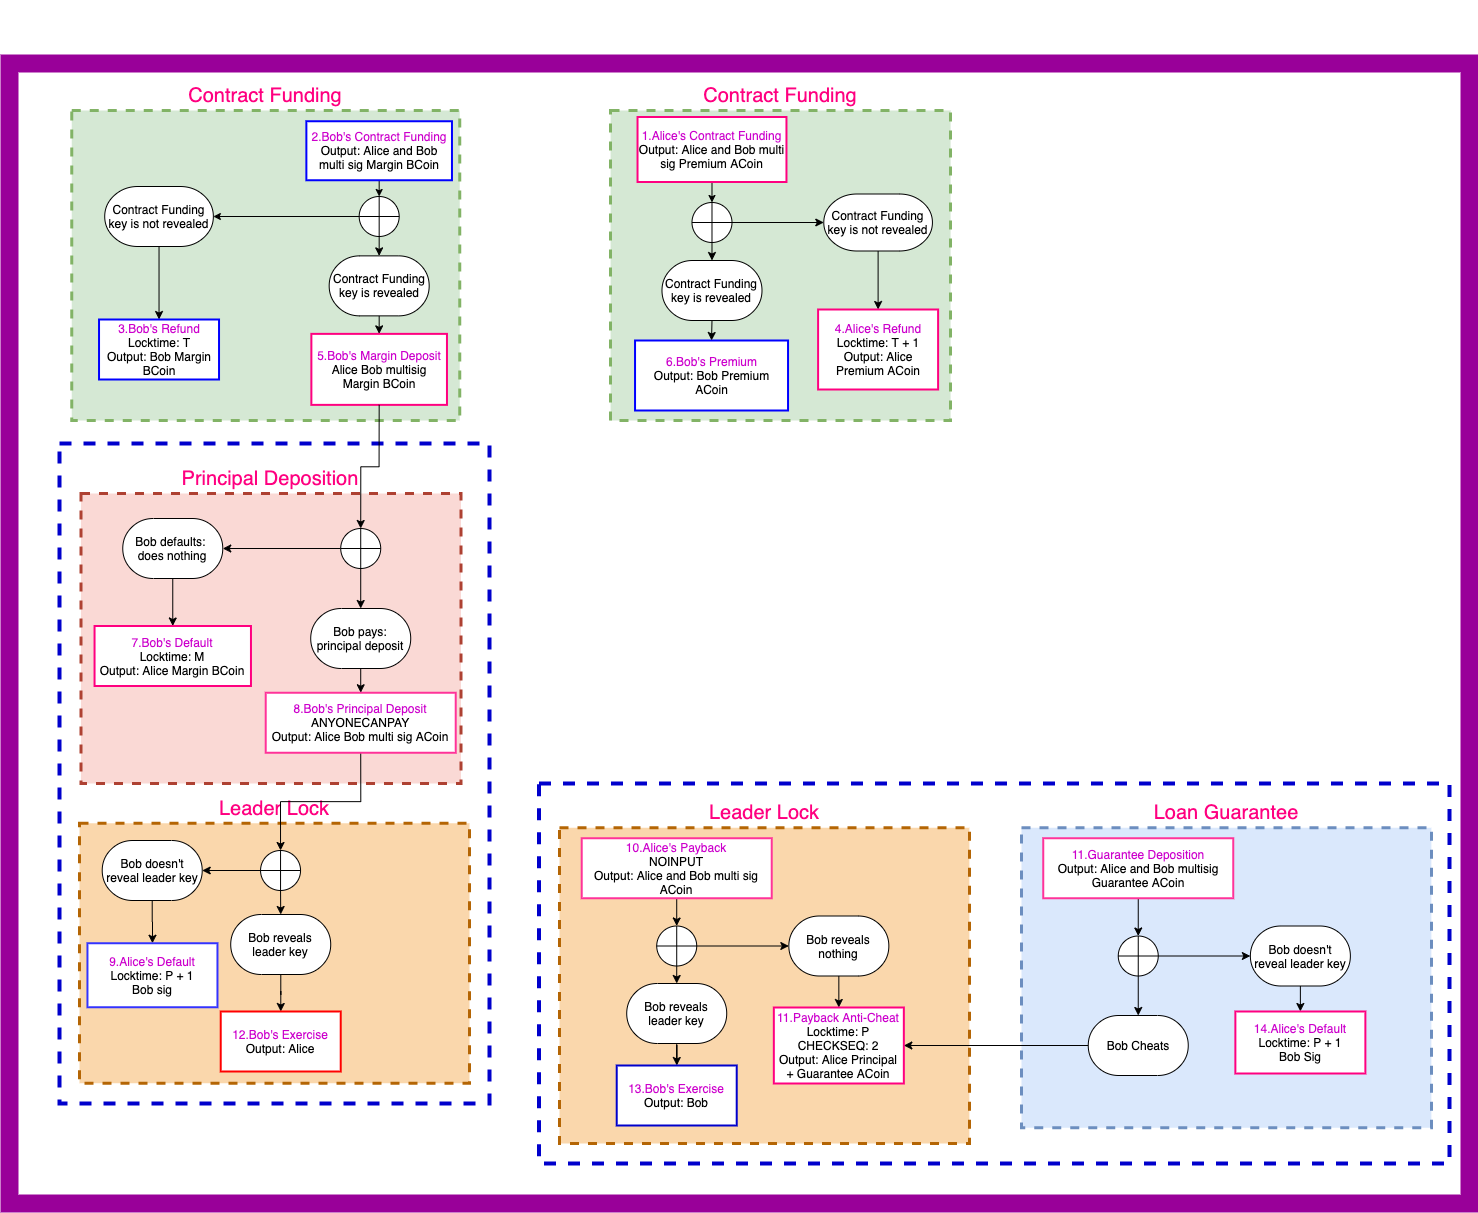
\includegraphics[width=\textwidth]{figures/non-collateralized-bond-checkseq-cross-chain.png}
    \caption{Crosschain Non-collateralized bond with CHECKSEQVERIFY}
    \label{fig:cross-chain-non-collat-bond}
\end{figure}